\documentclass[]{article}
\usepackage{lmodern}
\usepackage{amssymb,amsmath}
\usepackage{ifxetex,ifluatex}
\usepackage{fixltx2e} % provides \textsubscript
\ifnum 0\ifxetex 1\fi\ifluatex 1\fi=0 % if pdftex
  \usepackage[T1]{fontenc}
  \usepackage[utf8]{inputenc}
\else % if luatex or xelatex
  \ifxetex
    \usepackage{mathspec}
  \else
    \usepackage{fontspec}
  \fi
  \defaultfontfeatures{Ligatures=TeX,Scale=MatchLowercase}
\fi
% use upquote if available, for straight quotes in verbatim environments
\IfFileExists{upquote.sty}{\usepackage{upquote}}{}
% use microtype if available
\IfFileExists{microtype.sty}{%
\usepackage{microtype}
\UseMicrotypeSet[protrusion]{basicmath} % disable protrusion for tt fonts
}{}
\usepackage[margin=1in]{geometry}
\usepackage{hyperref}
\hypersetup{unicode=true,
            pdftitle={Supplementary Material for `Long-term use of cover crops reduces weed seedbanks'},
            pdfauthor={Nichols et al.~2020},
            pdfborder={0 0 0},
            breaklinks=true}
\urlstyle{same}  % don't use monospace font for urls
\usepackage{graphicx}
% grffile has become a legacy package: https://ctan.org/pkg/grffile
\IfFileExists{grffile.sty}{%
\usepackage{grffile}
}{}
\makeatletter
\def\maxwidth{\ifdim\Gin@nat@width>\linewidth\linewidth\else\Gin@nat@width\fi}
\def\maxheight{\ifdim\Gin@nat@height>\textheight\textheight\else\Gin@nat@height\fi}
\makeatother
% Scale images if necessary, so that they will not overflow the page
% margins by default, and it is still possible to overwrite the defaults
% using explicit options in \includegraphics[width, height, ...]{}
\setkeys{Gin}{width=\maxwidth,height=\maxheight,keepaspectratio}
\IfFileExists{parskip.sty}{%
\usepackage{parskip}
}{% else
\setlength{\parindent}{0pt}
\setlength{\parskip}{6pt plus 2pt minus 1pt}
}
\setlength{\emergencystretch}{3em}  % prevent overfull lines
\providecommand{\tightlist}{%
  \setlength{\itemsep}{0pt}\setlength{\parskip}{0pt}}
\setcounter{secnumdepth}{0}
% Redefines (sub)paragraphs to behave more like sections
\ifx\paragraph\undefined\else
\let\oldparagraph\paragraph
\renewcommand{\paragraph}[1]{\oldparagraph{#1}\mbox{}}
\fi
\ifx\subparagraph\undefined\else
\let\oldsubparagraph\subparagraph
\renewcommand{\subparagraph}[1]{\oldsubparagraph{#1}\mbox{}}
\fi

%%% Use protect on footnotes to avoid problems with footnotes in titles
\let\rmarkdownfootnote\footnote%
\def\footnote{\protect\rmarkdownfootnote}

%%% Change title format to be more compact
\usepackage{titling}

% Create subtitle command for use in maketitle
\providecommand{\subtitle}[1]{
  \posttitle{
    \begin{center}\large#1\end{center}
    }
}

\setlength{\droptitle}{-2em}

  \title{Supplementary Material for `Long-term use of cover crops reduces weed
seedbanks'}
    \pretitle{\vspace{\droptitle}\centering\huge}
  \posttitle{\par}
    \author{Nichols et al.~2020}
    \preauthor{\centering\large\emph}
  \postauthor{\par}
      \predate{\centering\large\emph}
  \postdate{\par}
    \date{7/15/2020}

\usepackage{booktabs}
\usepackage{longtable}
\usepackage{array}
\usepackage{multirow}
\usepackage{wrapfig}
\usepackage{float}
\usepackage{colortbl}
\usepackage{pdflscape}
\usepackage{tabu}
\usepackage{threeparttable}
\usepackage{threeparttablex}
\usepackage[normalem]{ulem}
\usepackage{makecell}
\usepackage{xcolor}

\usepackage{float}
\floatplacement{figure}{H}

\begin{document}
\maketitle

\hypertarget{general-site-management-summary}{%
\section{General Site Management
Summary}\label{general-site-management-summary}}

\begin{table}[H]

\caption{\label{tab:unnamed-chunk-1}General Site Description}
\centering
\begin{tabular}[t]{>{\centering\arraybackslash}p{3em}>{\centering\arraybackslash}p{7em}>{\centering\arraybackslash}p{5em}>{\centering\arraybackslash}p{5em}>{\centering\arraybackslash}p{5em}>{\centering\arraybackslash}p{5em}c}
\toprule
Site Description & General Location & Treatment Description & Year of Initiation & Crop Planted in 2019 & Number of Treatment Replicates & Sampled in 2019\\
\midrule
\rowcolor{gray!6}   & Boyd Farm, Boone, field 44 & corn/soybean grain rotation, with and without rye cover crop & 2009 & corn & 5 & Y\\

\multirow{-2}{*}{\centering\arraybackslash Central Grain} & Boyd Farm, Boone, field 42 & corn/soybean grain rotation, with and without rye cover crop & 2009 & soy & 5 & Y\\
\cmidrule{1-7}
\rowcolor{gray!6}   & Boyd Farm, Boone, field 44 & corn silage/soybean grain rotation, with and without rye cover crop & 2002 & corn silage & 5 & Y\\

\multirow{-2}{*}{\centering\arraybackslash Central Silage} & Boyd Farm, Boone, field 42 & corn silage/soybean grain rotation, with and without rye cover crop & 2002 & soy & 5 & N\\
\cmidrule{1-7}
\rowcolor{gray!6}  West & Jefferson, IA & corn/soybean grain rotation, with and without rye cover crop & 2008 & corn & 4 & Y\\
\cmidrule{1-7}
East & Washington, IA & corn/soybean grain rotation, with and without rye cover crop & 2009 & soybeans & 4 & Y\\
\bottomrule
\end{tabular}
\end{table}

\newpage

\begin{table}[H]

\caption{\label{tab:unnamed-chunk-2}2018-2019 Herbicide Use}
\centering
\begin{tabular}[t]{>{\centering\arraybackslash}p{8em}>{\centering\arraybackslash}p{8em}>{\centering\arraybackslash}p{8em}>{\centering\arraybackslash}p{8em}}
\toprule
Site Description & Herbicides Used in 2018 Growing Season & Herbicdes Used in Fall 2018 & Herbicides Used in Spring 2019\\
\midrule
\rowcolor{gray!6}   & glyphosate 1 week before soybean planting & none & glyphosate 1 week before corn planting, Lumax at planting\\

\multirow{-2}{8em}{\centering\arraybackslash Central Grain} & glyphosate 1 week before corn planting, Lumax at planting & none & glyphosate 1 week before soybean planting\\
\cmidrule{1-4}
\rowcolor{gray!6}   & glyphosate 1 week before soybean planting & none & glyphosate 1 week before corn planting, Lumax at planting\\

\multirow{-2}{8em}{\centering\arraybackslash Central Silage} & glyphosate 1 week before corn planting, Lumax at planting & none & glyphosate 1 week before soybean planting\\
\cmidrule{1-4}
\rowcolor{gray!6}  West & Roundup and Cadet & none & Roundup and Cadet\\
\cmidrule{1-4}
East & April 15-Roundup Powermax 32 oz; April 15-Acetochlor ATZ 40 oz; May 14-Aatrex 9-0   1/2; May 14-Harness Max  40 oz; June 15-Warrant Ultra 50 oz; June 15-Roundup Powermax 22 oz; & none & 3 oz Fierce XLT  with 26-32 oz Roundup Powermax as burndown followed by a post emergence application of 22 oz Xtendimax plus 2 pt of Warrant\\
\bottomrule
\end{tabular}
\end{table}

\newpage

\begin{table}[H]

\caption{\label{tab:unnamed-chunk-3}General Management}
\centering
\begin{tabular}[t]{c>{\centering\arraybackslash}p{7em}>{\centering\arraybackslash}p{5em}>{\centering\arraybackslash}p{5em}>{\centering\arraybackslash}p{5em}>{\centering\arraybackslash}p{5em}>{\centering\arraybackslash}p{5em}}
\toprule
Site Description & General Herbicide Regime & General Date of Cover Crop Termination & General Date of Crop Planting & Inorganic Fertilizer Used & Organic Fertilizer Used & Tillage Used\\
\midrule
\rowcolor{gray!6}   & burndown, residual herbicide at corn planting & 15-Apr & 26-Apr & Y & NA & N\\

\multirow{-2}{*}{\centering\arraybackslash Central Grain} & burndown, residual herbicide at corn planting & 25-Apr & 5-May & Y & NA & N\\
\cmidrule{1-7}
\rowcolor{gray!6}   & burndown, residual herbicide at corn planting & 15-Apr & 26-Apr & Y & NA & N\\

\multirow{-2}{*}{\centering\arraybackslash Central Silage} & burndown, residual herbicide at corn planting & 25-Apr & 5-May & Y & NA & N\\
\cmidrule{1-7}
\rowcolor{gray!6}  West & burndown, pre-emergent herbicide & 1-May & 10-May & Y & chicken/turkey manure & N\\
\cmidrule{1-7}
East & burndown, residual herbicide at planting, another application on corn at \textasciitilde{}V6 & 1-May & 5-May & Y & liquid swine, \textasciitilde{}3000 gal/ac every other year to entire field & N\\
\bottomrule
\end{tabular}
\end{table}

\newpage

\hypertarget{field-wet-soil-amounts}{%
\section{Field wet soil amounts}\label{field-wet-soil-amounts}}

\begin{table}[H]

\caption{\label{tab:unnamed-chunk-4}Wet Soil Weights Immediately After Sampling}
\centering
\begin{tabular}[t]{ccccc}
\toprule
site & cc\_trt & rep & soilwt\_g & notes\\
\midrule
\rowcolor{gray!6}   & no & 1 & 6718.3 & sampled 4/8, 12-6pm\\

 & rye & 1 & 6936.2 & sampled 4/8, 12-6pm\\

\rowcolor{gray!6}   & no & 2 & 6838.6 & sampled 4/8, 12-6pm\\

 & rye & 2 & 5965.2 & sampled 4/8, 12-6pm\\

\rowcolor{gray!6}   & no & 3 & 6260.4 & sampled 4/8, 12-6pm\\

 & rye & 3 & 6136.0 & sampled 4/8, 12-6pm\\

\rowcolor{gray!6}   & no & 4 & 5554.9 & sampled 4/9\\

 & rye & 4 & 6312.7 & sampled 4/9\\

\rowcolor{gray!6}   & no & 5 & 5866.2 & sampled 4/9\\

\multirow[t]{-10}{*}{\centering\arraybackslash BC} & rye & 5 & 5981.1 & sampled 4/9\\
\cmidrule{1-5}
\rowcolor{gray!6}   & rye & 1 & 6340.0 & sampled 4/16, 2-6pm\\

 & no & 1 & 5800.0 & sampled 4/16, 2-6pm\\

\rowcolor{gray!6}   & rye & 2 & 5990.0 & sampled 4/16, 2-6pm\\

 & no & 2 & 6100.0 & sampled 4/16, 2-6pm\\

\rowcolor{gray!6}   & no & 3 & 6245.5 & sampled 4/8\\

 & rye & 3 & 6160.2 & sampled 4/8\\

\rowcolor{gray!6}   & no & 4 & 6240.2 & sampled 4/8\\

 & rye & 4 & 6007.5 & sampled 4/8\\

\rowcolor{gray!6}   & no & 5 & 6682.9 & sampled 4/8\\

\multirow[t]{-10}{*}{\centering\arraybackslash Bcsil} & rye & 5 & 6045.7 & sampled 4/8\\
\cmidrule{1-5}
\rowcolor{gray!6}   & rye & 1 & 6068.7 & sampled 4/9\\

 & no & 2 & 6240.3 & sampled 4/9\\

\rowcolor{gray!6}   & rye & 2 & 5950.5 & sampled 4/9\\

 & no & 3 & 5885.7 & sampled 4/9\\

\rowcolor{gray!6}   & rye & 3 & 5734.1 & sampled 4/9\\

 & no & 4 & 6213.3 & sampled 4/9\\

\rowcolor{gray!6}   & rye & 4 & 5968.2 & sampled 4/9\\

 & no & 5 & 6175.8 & sampled 4/9\\

\rowcolor{gray!6}  \multirow[t]{-9}{*}{\centering\arraybackslash BS} & rye & 5 & 6050.4 & sampled 4/9\\
\cmidrule{1-5}
 & no & 1 & 5349.6 & sampled 4/6, 8-5pm\\

\rowcolor{gray!6}   & rye & 1 & 5460.6 & sampled 4/6, 8-5pm\\

 & no & 2 & 5235.5 & sampled 4/6, 8-5pm\\

\rowcolor{gray!6}   & rye & 2 & 5055.2 & sampled 4/6, 8-5pm\\

 & no & 3 & 5211.1 & sampled 4/6, 8-5pm\\

\rowcolor{gray!6}   & rye & 3 & 4991.7 & sampled 4/6, 8-5pm\\

 & no & 4 & 5401.6 & sampled 4/6, 8-5pm\\

\rowcolor{gray!6}  \multirow[t]{-8}{*}{\centering\arraybackslash East} & rye & 4 & 5163.9 & sampled 4/6, 8-5pm\\
\cmidrule{1-5}
 & no & 1 & 6314.0 & sampled 4/17, 9-2pm\\

\rowcolor{gray!6}   & rye & 1 & 6401.0 & sampled 4/17, 9-2pm\\

 & no & 2 & 5841.0 & sampled 4/17, 9-2pm\\

\rowcolor{gray!6}   & rye & 2 & 5543.0 & sampled 4/17, 9-2pm\\

 & no & 3 & 5698.0 & sampled 4/17, 9-2pm\\

\rowcolor{gray!6}   & rye & 3 & 5947.0 & sampled 4/17, 9-2pm\\

 & no & 4 & 6057.0 & sampled 4/17, 9-2pm\\

\rowcolor{gray!6}  \multirow[t]{-8}{*}{\centering\arraybackslash West} & rye & 4 & 5989.0 & sampled 4/17, 9-2pm\\
\bottomrule
\end{tabular}
\end{table}

\newpage

\hypertarget{statistical-results}{%
\section{Statistical Results}\label{statistical-results}}

\emph{Note: Boyd refers to the Central site, Stout to the East site, and
Funcke to the West site}

\hypertarget{linear-models-on-seedbank-density}{%
\subsection{Linear models on seedbank
density}\label{linear-models-on-seedbank-density}}

Values are presented for the models run with the full dataset (XX\_full)
and with the outlier removed (XX\_out-rm)

\begin{table}[H]

\caption{\label{tab:unnamed-chunk-5}Contrasts using full dataset (full) and dataset with outlier removed (out-rm)}
\centering
\begin{tabular}[t]{cccccccc}
\toprule
model & site\_sys & level1 & level2 & estimate & std.error & z.ratio & p.value\\
\midrule
\rowcolor{gray!6}   & Boyd\_grain & no & rye & -0.32 & 0.26 & -1.22 & 0.22\\

 & Boyd\_silage & no & rye & 0.95 & 0.35 & 2.66 & 0.01\\

\rowcolor{gray!6}   & Funcke\_grain & no & rye & 0.71 & 0.42 & 1.68 & 0.09\\

\multirow{-4}{*}{\centering\arraybackslash pois\_out-rm} & Stout\_grain & no & rye & 0.42 & 0.41 & 1.03 & 0.31\\
\cmidrule{1-8}
\rowcolor{gray!6}   & Boyd\_grain & no & rye & -0.32 & 0.27 & -1.19 & 0.24\\

 & Boyd\_silage & no & rye & 0.95 & 0.37 & 2.58 & 0.01\\

\rowcolor{gray!6}   & Funcke\_grain & no & rye & 0.36 & 0.40 & 0.91 & 0.37\\

\multirow{-4}{*}{\centering\arraybackslash pois\_full} & Stout\_grain & no & rye & 0.43 & 0.43 & 1.00 & 0.32\\
\cmidrule{1-8}
\rowcolor{gray!6}   & Boyd\_grain & no & rye & -0.33 & 0.26 & -1.27 & 0.20\\

 & Boyd\_silage & no & rye & 1.02 & 0.34 & 2.99 & 0.00\\

\rowcolor{gray!6}   & Funcke\_grain & no & rye & 0.71 & 0.41 & 1.72 & 0.09\\

\multirow{-4}{*}{\centering\arraybackslash binom\_out-rm} & Stout\_grain & no & rye & 0.45 & 0.40 & 1.12 & 0.26\\
\cmidrule{1-8}
\rowcolor{gray!6}   & Boyd\_grain & no & rye & -0.33 & 0.26 & -1.23 & 0.22\\

 & Boyd\_silage & no & rye & 1.03 & 0.35 & 2.92 & 0.00\\

\rowcolor{gray!6}   & Funcke\_grain & no & rye & 0.28 & 0.39 & 0.71 & 0.48\\

\multirow{-4}{*}{\centering\arraybackslash binom\_full} & Stout\_grain & no & rye & 0.45 & 0.41 & 1.09 & 0.27\\
\bottomrule
\end{tabular}
\end{table}

\begin{table}[H]

\caption{\label{tab:unnamed-chunk-6}Estimates using full dataset (full) and dataset with outlier removed (out-rm)}
\centering
\begin{tabular}[t]{ccccccc}
\toprule
model & site\_sys & cc\_trt & estimate & std.error & asymp.LCL & asymp.UCL\\
\midrule
\rowcolor{gray!6}   &  & no & 2.97 & 0.23 & 2.52 & 3.42\\

 & \multirow{-2}{*}{\centering\arraybackslash Boyd\_grain} & rye & 3.29 & 0.23 & 2.85 & 3.73\\

\rowcolor{gray!6}   &  & no & 4.30 & 0.30 & 3.72 & 4.88\\

 & \multirow{-2}{*}{\centering\arraybackslash Boyd\_silage} & rye & 3.35 & 0.30 & 2.76 & 3.95\\

\rowcolor{gray!6}   &  & no & 6.02 & 0.34 & 5.35 & 6.69\\

 & \multirow{-2}{*}{\centering\arraybackslash Funcke\_grain} & rye & 5.31 & 0.39 & 4.55 & 6.07\\

\rowcolor{gray!6}   &  & no & 3.32 & 0.36 & 2.62 & 4.03\\

\multirow{-8}{*}{\centering\arraybackslash pois\_out-rm} & \multirow{-2}{*}{\centering\arraybackslash Stout\_grain} & rye & 2.90 & 0.36 & 2.19 & 3.61\\
\cmidrule{1-7}
\rowcolor{gray!6}   &  & no & 2.97 & 0.24 & 2.50 & 3.43\\

 & \multirow{-2}{*}{\centering\arraybackslash Boyd\_grain} & rye & 3.29 & 0.23 & 2.83 & 3.74\\

\rowcolor{gray!6}   &  & no & 4.29 & 0.31 & 3.69 & 4.90\\

 & \multirow{-2}{*}{\centering\arraybackslash Boyd\_silage} & rye & 3.35 & 0.31 & 2.74 & 3.96\\

\rowcolor{gray!6}   &  & no & 6.02 & 0.35 & 5.33 & 6.71\\

 & \multirow{-2}{*}{\centering\arraybackslash Funcke\_grain} & rye & 5.66 & 0.36 & 4.97 & 6.36\\

\rowcolor{gray!6}   &  & no & 3.32 & 0.37 & 2.60 & 4.05\\

\multirow{-8}{*}{\centering\arraybackslash pois\_full} & \multirow{-2}{*}{\centering\arraybackslash Stout\_grain} & rye & 2.90 & 0.38 & 2.16 & 3.63\\
\cmidrule{1-7}
\rowcolor{gray!6}   &  & no & 3.11 & 0.23 & 2.67 & 3.55\\

 & \multirow{-2}{*}{\centering\arraybackslash Boyd\_grain} & rye & 3.44 & 0.23 & 3.00 & 3.88\\

\rowcolor{gray!6}   &  & no & 4.45 & 0.29 & 3.87 & 5.02\\

 & \multirow{-2}{*}{\centering\arraybackslash Boyd\_silage} & rye & 3.42 & 0.30 & 2.84 & 4.01\\

\rowcolor{gray!6}   &  & no & 6.03 & 0.33 & 5.37 & 6.68\\

 & \multirow{-2}{*}{\centering\arraybackslash Funcke\_grain} & rye & 5.32 & 0.38 & 4.58 & 6.06\\

\rowcolor{gray!6}   &  & no & 3.43 & 0.36 & 2.73 & 4.13\\

\multirow{-8}{*}{\centering\arraybackslash binom\_out-rm} & \multirow{-2}{*}{\centering\arraybackslash Stout\_grain} & rye & 2.98 & 0.36 & 2.28 & 3.69\\
\cmidrule{1-7}
\rowcolor{gray!6}   &  & no & 3.11 & 0.23 & 2.65 & 3.57\\

 & \multirow{-2}{*}{\centering\arraybackslash Boyd\_grain} & rye & 3.43 & 0.24 & 2.97 & 3.90\\

\rowcolor{gray!6}   &  & no & 4.44 & 0.30 & 3.85 & 5.04\\

 & \multirow{-2}{*}{\centering\arraybackslash Boyd\_silage} & rye & 3.42 & 0.31 & 2.81 & 4.02\\

\rowcolor{gray!6}   &  & no & 6.04 & 0.35 & 5.35 & 6.72\\

 & \multirow{-2}{*}{\centering\arraybackslash Funcke\_grain} & rye & 5.76 & 0.36 & 5.06 & 6.46\\

\rowcolor{gray!6}   &  & no & 3.42 & 0.37 & 2.69 & 4.15\\

\multirow{-8}{*}{\centering\arraybackslash binom\_full} & \multirow{-2}{*}{\centering\arraybackslash Stout\_grain} & rye & 2.98 & 0.37 & 2.24 & 3.71\\
\bottomrule
\end{tabular}
\end{table}

\hypertarget{biomass-metrics}{%
\subsection{Biomass metrics}\label{biomass-metrics}}

\begin{table}[H]

\caption{\label{tab:unnamed-chunk-7}Cover crop biomass metrics}
\centering
\begin{tabular}[t]{cccccccccc}
\toprule
site\_sys & yr\_span & nabove1 & nabove2 & ccbio\_mean & ccbio\_med & ccbio\_var & ccbio\_max & ccbio\_stab & ccbio\_2019\\
\midrule
\rowcolor{gray!6}  Boyd\_grain &  & 4 & 2 & 1.03 & 0.74 & 0.77 & 2.76 & 0.85 & 1.29\\

Boyd\_silage &  & 9 & 4 & 2.04 & 1.74 & 1.02 & 4.23 & 0.50 & 2.05\\

\rowcolor{gray!6}  Funcke\_grain &  & 2 & 1 & 0.45 & 0.14 & 0.46 & 2.11 & 1.50 & 0.00\\

Stout\_grain & \multirow{-4}{*}{\centering\arraybackslash 10yr} & 3 & 2 & 1.32 & 0.43 & 4.89 & 7.30 & 1.68 & 0.30\\
\cmidrule{1-10}
\rowcolor{gray!6}  Boyd\_grain &  & 3 & 2 & 1.72 & 1.76 & 0.91 & 2.76 & 0.55 & 1.29\\

Boyd\_silage &  & 4 & 3 & 2.56 & 2.13 & 1.27 & 4.23 & 0.44 & 2.05\\

\rowcolor{gray!6}  Funcke\_grain &  & 0 & 0 & 0.24 & 0.09 & 0.08 & 0.63 & 1.16 & 0.00\\

Stout\_grain & \multirow{-4}{*}{\centering\arraybackslash 5yr} & 1 & 1 & 1.73 & 0.36 & 9.71 & 7.30 & 1.80 & 0.30\\
\bottomrule
\end{tabular}
\end{table}

\begin{figure}
\centering
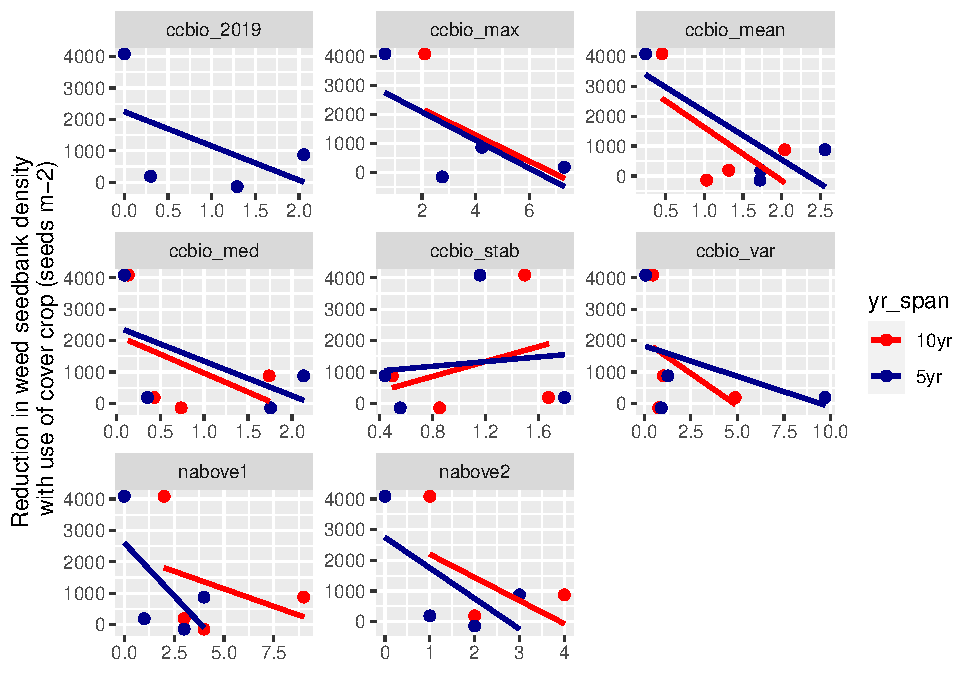
\includegraphics{supp-mat_files/figure-latex/unnamed-chunk-8-1.pdf}
\caption{Absolute Change in Seedbank Density vs.~Cover Crop Biomass
Metrics}
\end{figure}

\begin{figure}
\centering
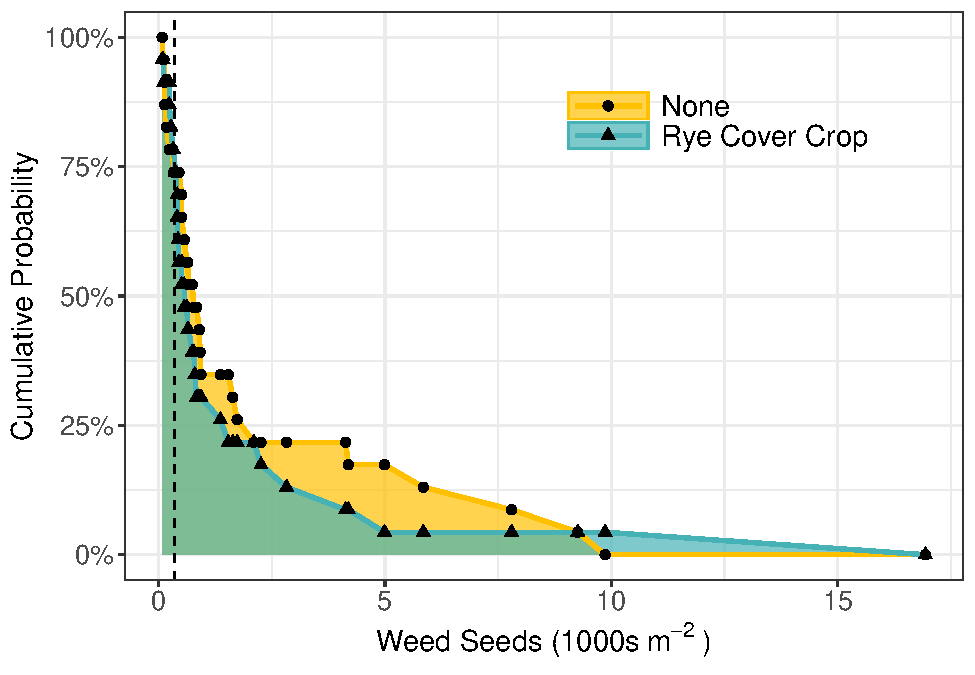
\includegraphics{supp-mat_files/figure-latex/unnamed-chunk-9-1.pdf}
\caption{Relative Change in Seedbank Density vs.~Cover Crop Biomass
Metrics}
\end{figure}

\newpage

\hypertarget{manuscript-figures-with-full-datasets}{%
\subsection{Manuscript figures with full
datasets}\label{manuscript-figures-with-full-datasets}}

\begin{figure}
\centering
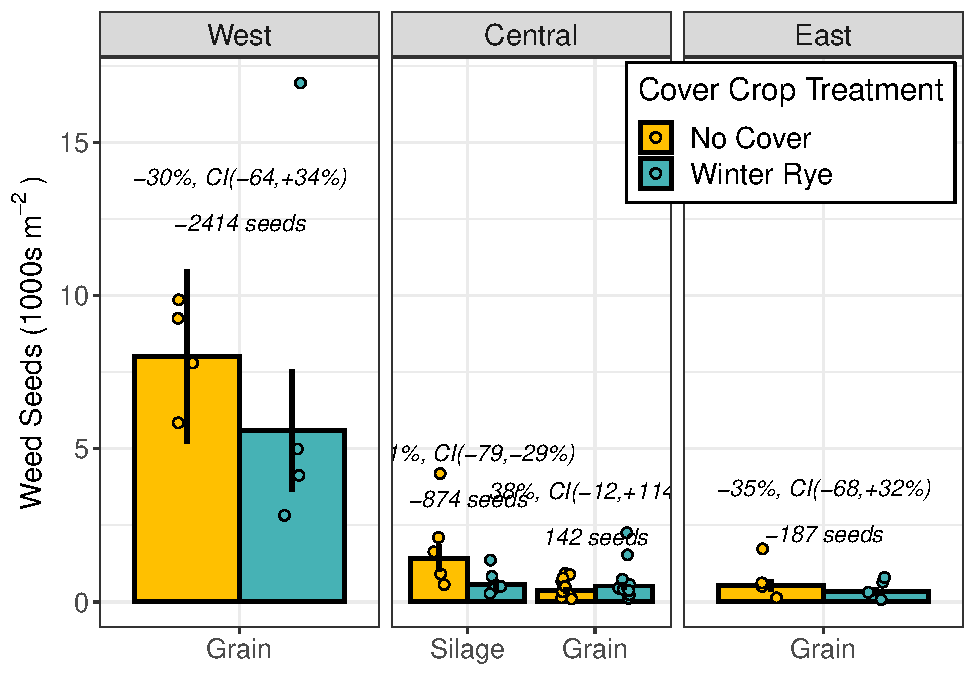
\includegraphics{supp-mat_files/figure-latex/unnamed-chunk-10-1.pdf}
\caption{Figure 2 on full dataset}
\end{figure}

\begin{figure}
\centering
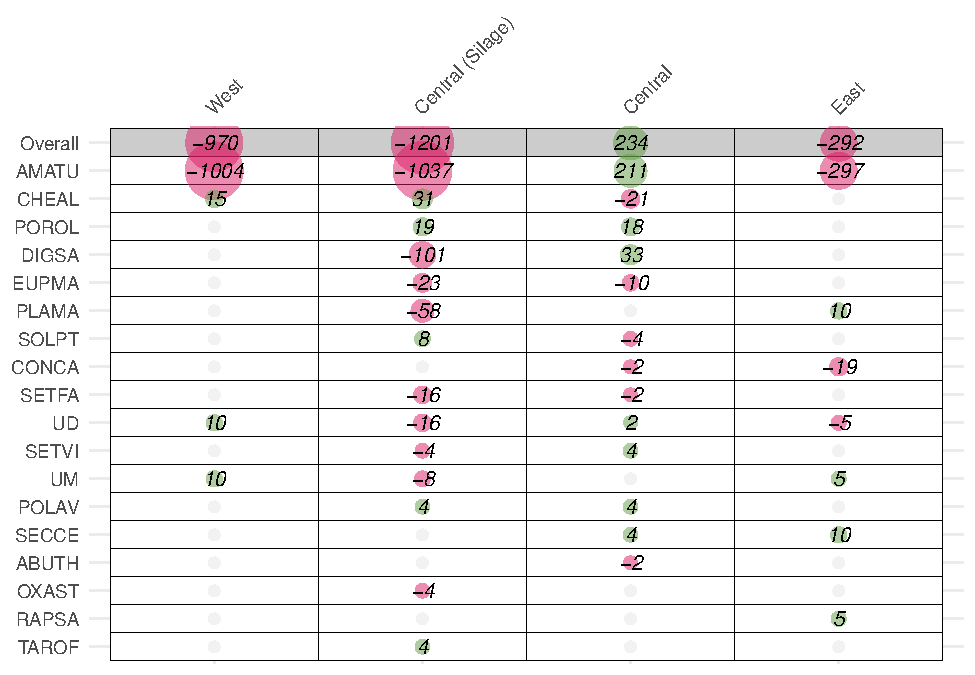
\includegraphics{supp-mat_files/figure-latex/unnamed-chunk-11-1.pdf}
\caption{Figure 4 using full dataset}
\end{figure}

\newpage

\begin{figure}
\centering
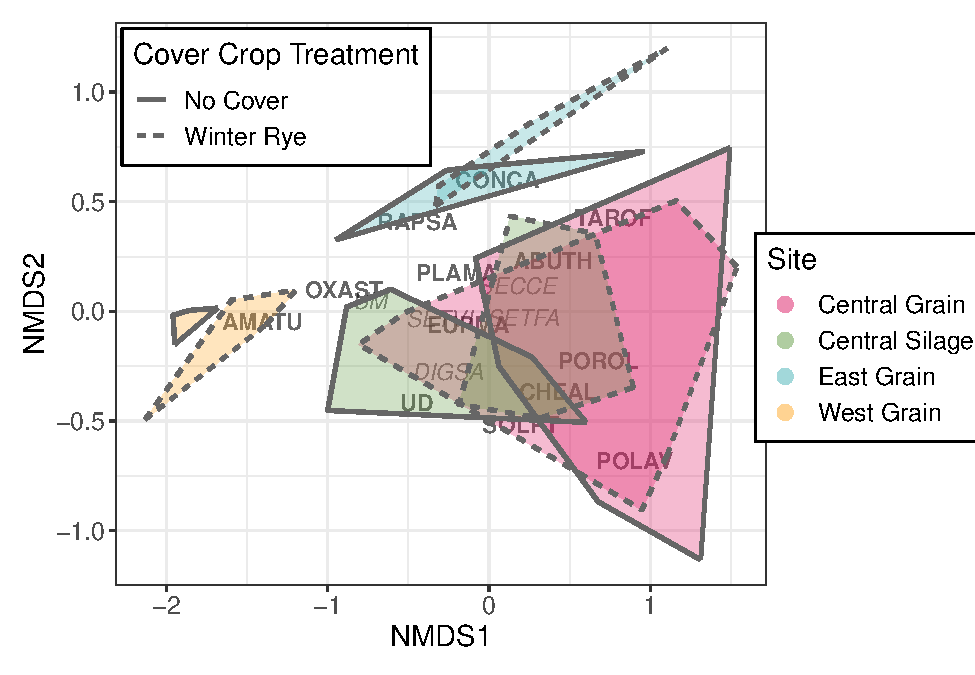
\includegraphics{supp-mat_files/figure-latex/unnamed-chunk-12-1.pdf}
\caption{Figure 4 on full dataset}
\end{figure}

\newpage

\begin{figure}
\centering
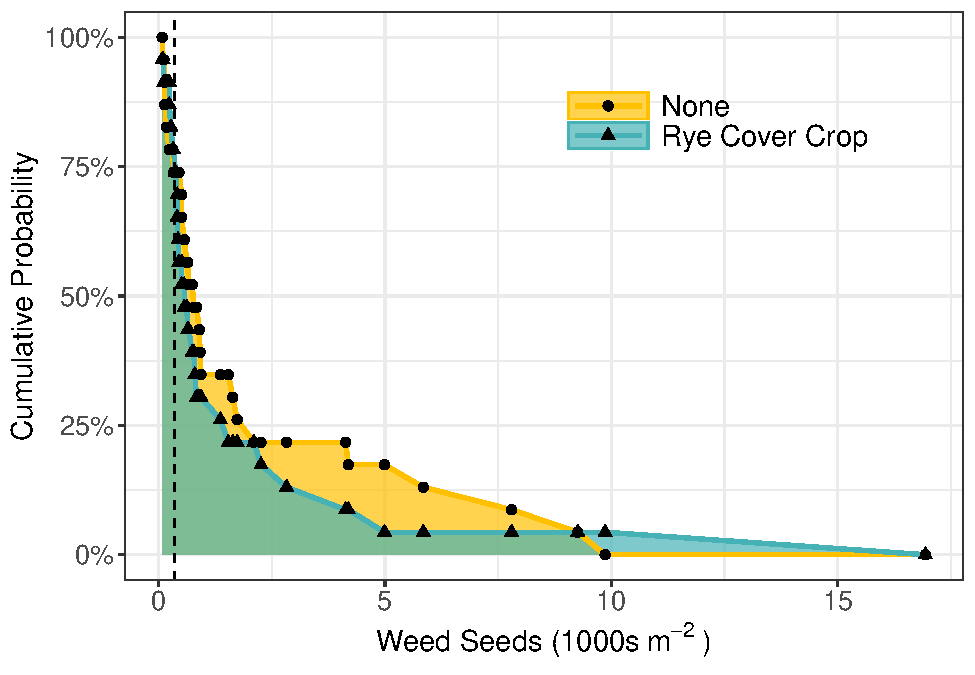
\includegraphics{supp-mat_files/figure-latex/unnamed-chunk-13-1.pdf}
\caption{Figure 5 on full dataset}
\end{figure}


\end{document}
